\chapter{System Architecture and Topology}
\label{chap:architecture}

\section{Overall Architecture Overview}
The College Campus Management System implements a multi-tier, serverless cloud architecture on Amazon Web Services. By decoupling presentation, API compute, persistence, notification, and authentication layers, the system achieves maximum elasticity and fault tolerance without relying on virtual machines.

Figure~\ref{fig:sys_arch} illustrates the complete end-to-end cloud architecture topology.

\begin{figure}[htbp]
\centering
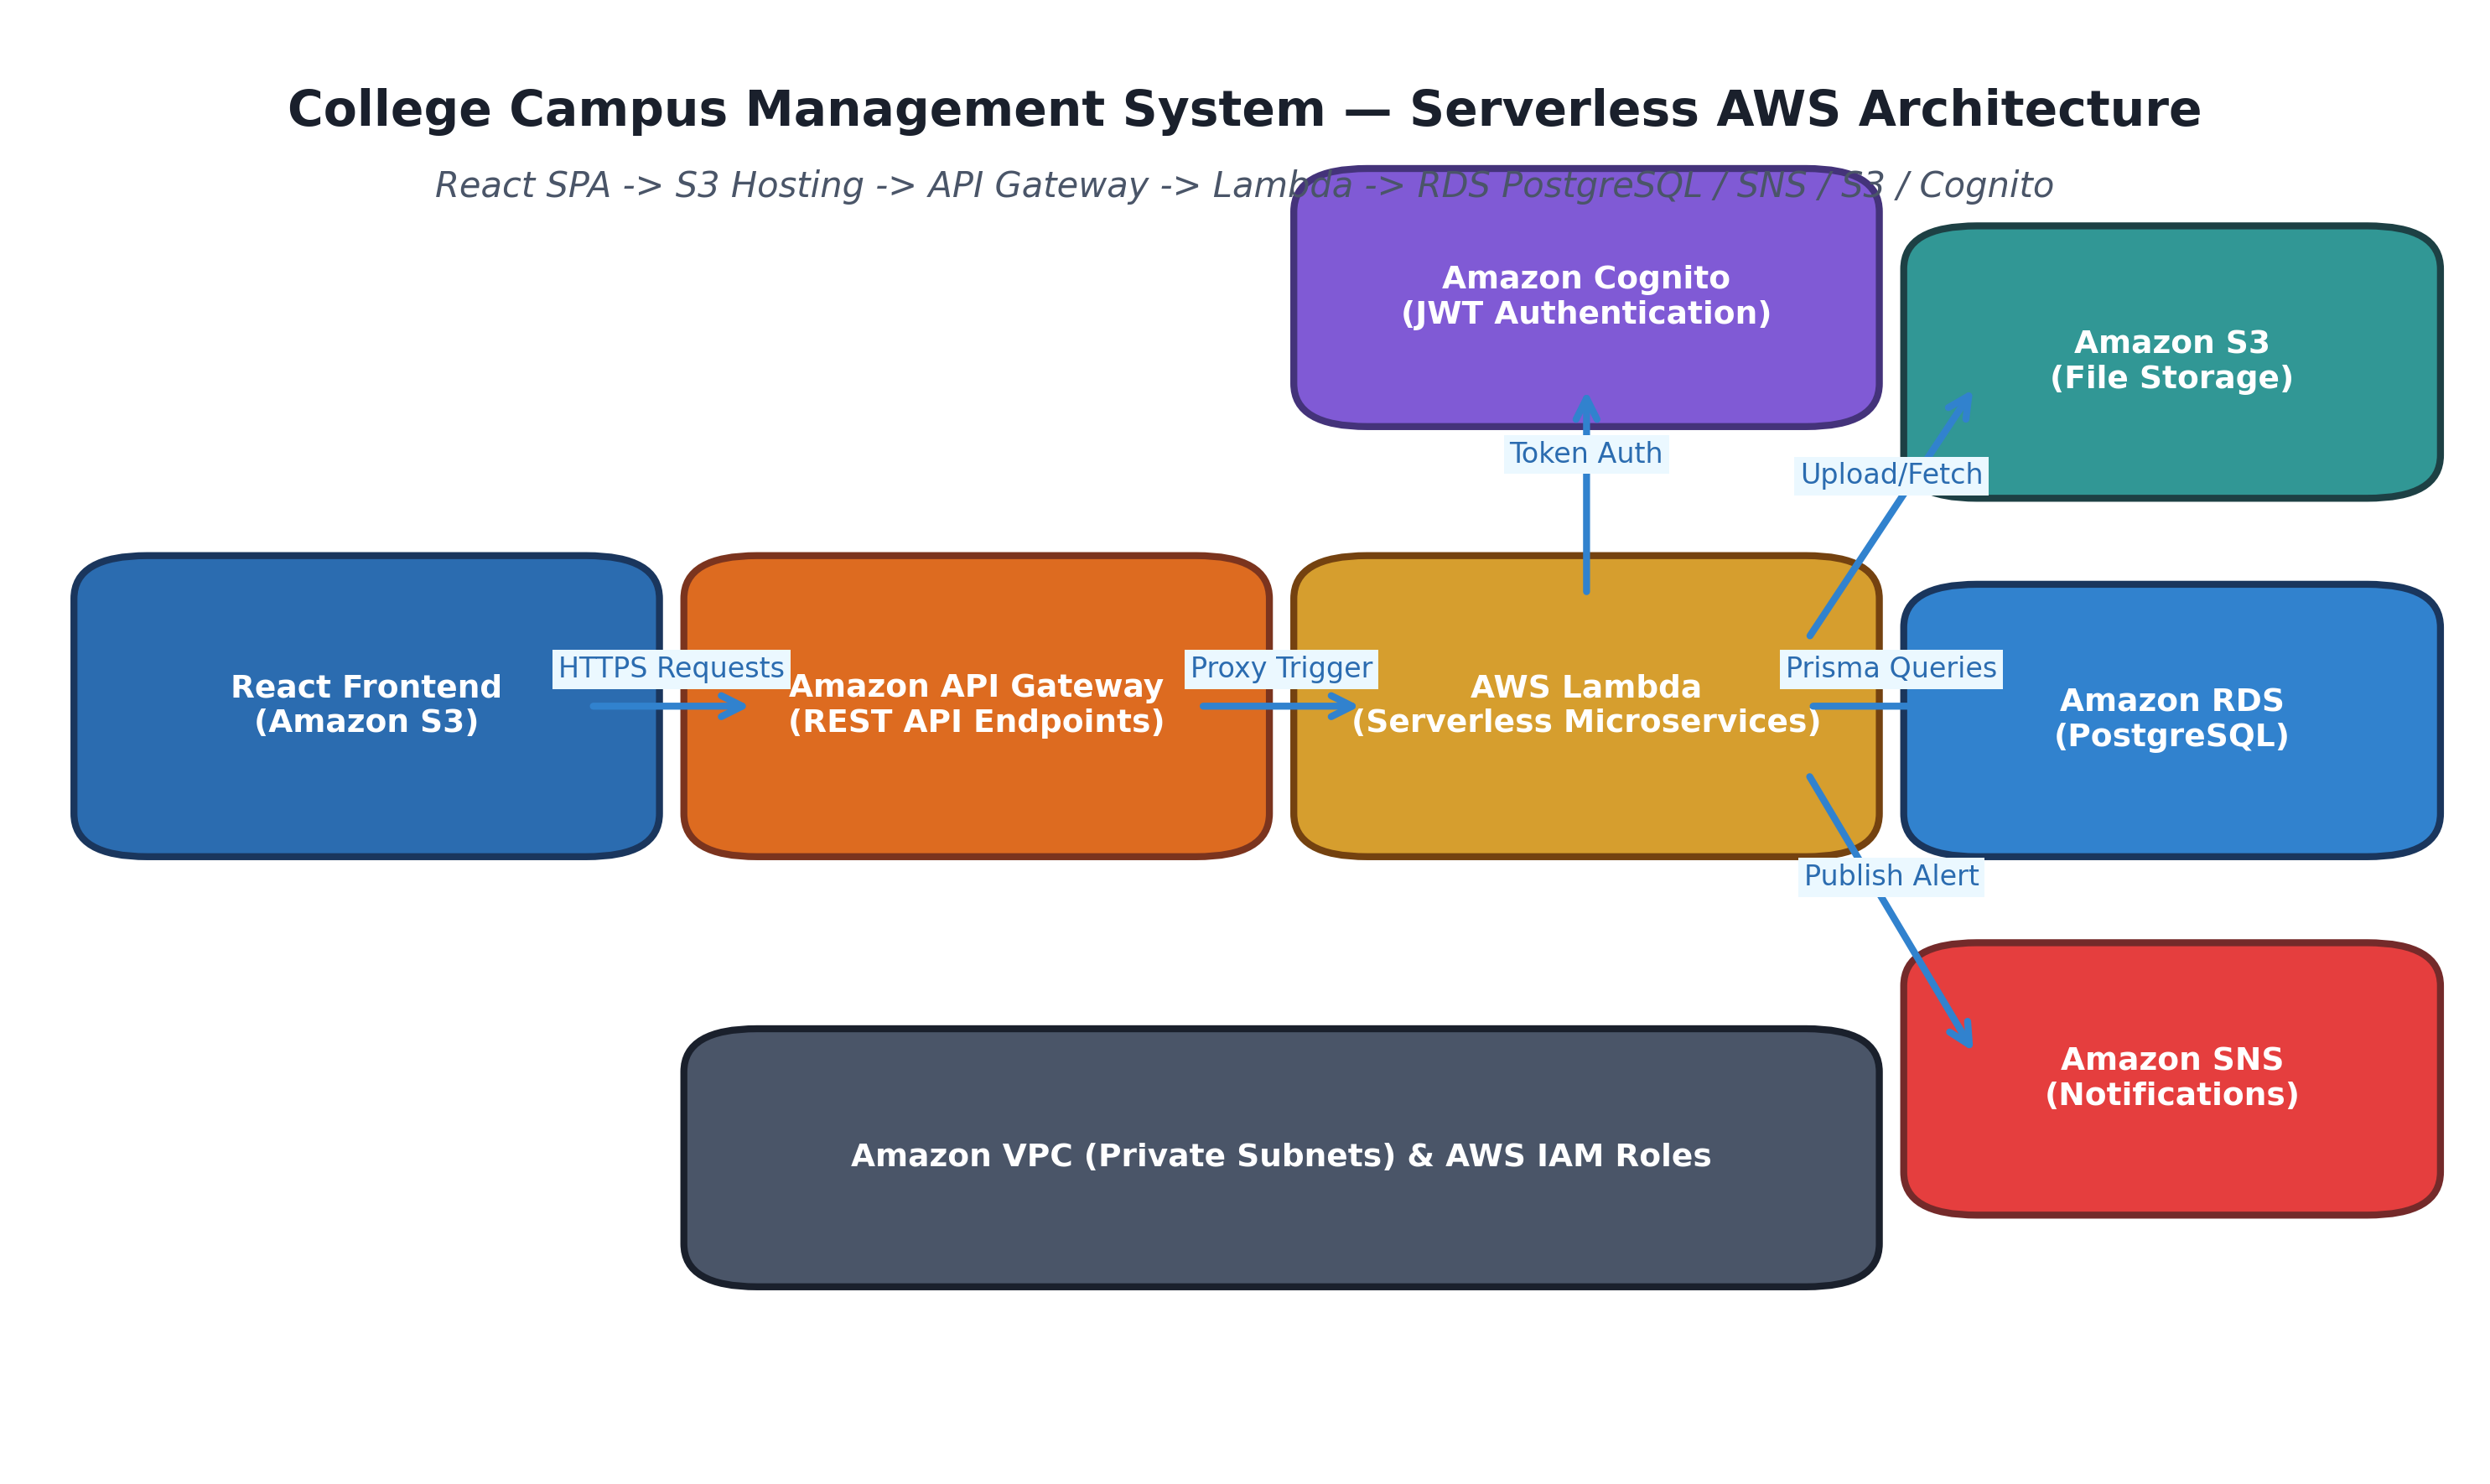
\includegraphics[width=0.92\textwidth]{figures/system_architecture.png}
\caption{Overall Cloud Architecture Topology for College Campus Management System}
\label{fig:sys_arch}
\end{figure}

\section{Component Tier Breakdown}

\subsection{Presentation Tier (Frontend)}
The presentation layer is a Single Page Application built with React 18, TypeScript, and Tailwind CSS. The compiled static assets (\texttt{index.html}, JavaScript bundles, CSS stylesheets) are hosted in an Amazon S3 bucket (\texttt{cloudcampus-frontend-static}) configured for Static Website Hosting. S3 delivers assets over HTTPS directly to client web browsers.

\subsection{API Gateway and Compute Tier (Backend)}
Client HTTP requests originating from the React SPA are routed to Amazon API Gateway. API Gateway acts as the single entry point, performing URL routing, CORS pre-flight validation, and rate limiting. Requests are proxied to an AWS Lambda function running Node.js 20.x and Express serverless middleware. Lambda executes application business logic and returns structured JSON responses.

\subsection{Persistence Tier (Database and Object Storage)}
Structured relational data is persisted in Amazon RDS for PostgreSQL 15.3, located within private VPC subnets. The backend accesses PostgreSQL via Prisma ORM using connection pooling. Unstructured files (assignment PDFs, syllabi) are stored directly in an Amazon S3 storage bucket.

\subsection{Authentication and Messaging Tier}
User identity authentication is managed via Amazon Cognito User Pools issuing RSA-256 signed JWT tokens. Asynchronous event alerts (exam announcements, grade postings) are published by Lambda to Amazon SNS topics, which handle email and push notifications.

\subsection{Security and Management Tier}
AWS IAM defines fine-grained access execution roles for Lambda. Amazon VPC encloses the RDS database and Lambda network interfaces inside private subnets, preventing direct internet exposure. Amazon CloudWatch ingests log streams and metrics.

\section{AWS Service Communication Topology}
Figure~\ref{fig:service_rel} shows the inter-service communication and security boundaries within the AWS ecosystem.

\begin{figure}[htbp]
\centering
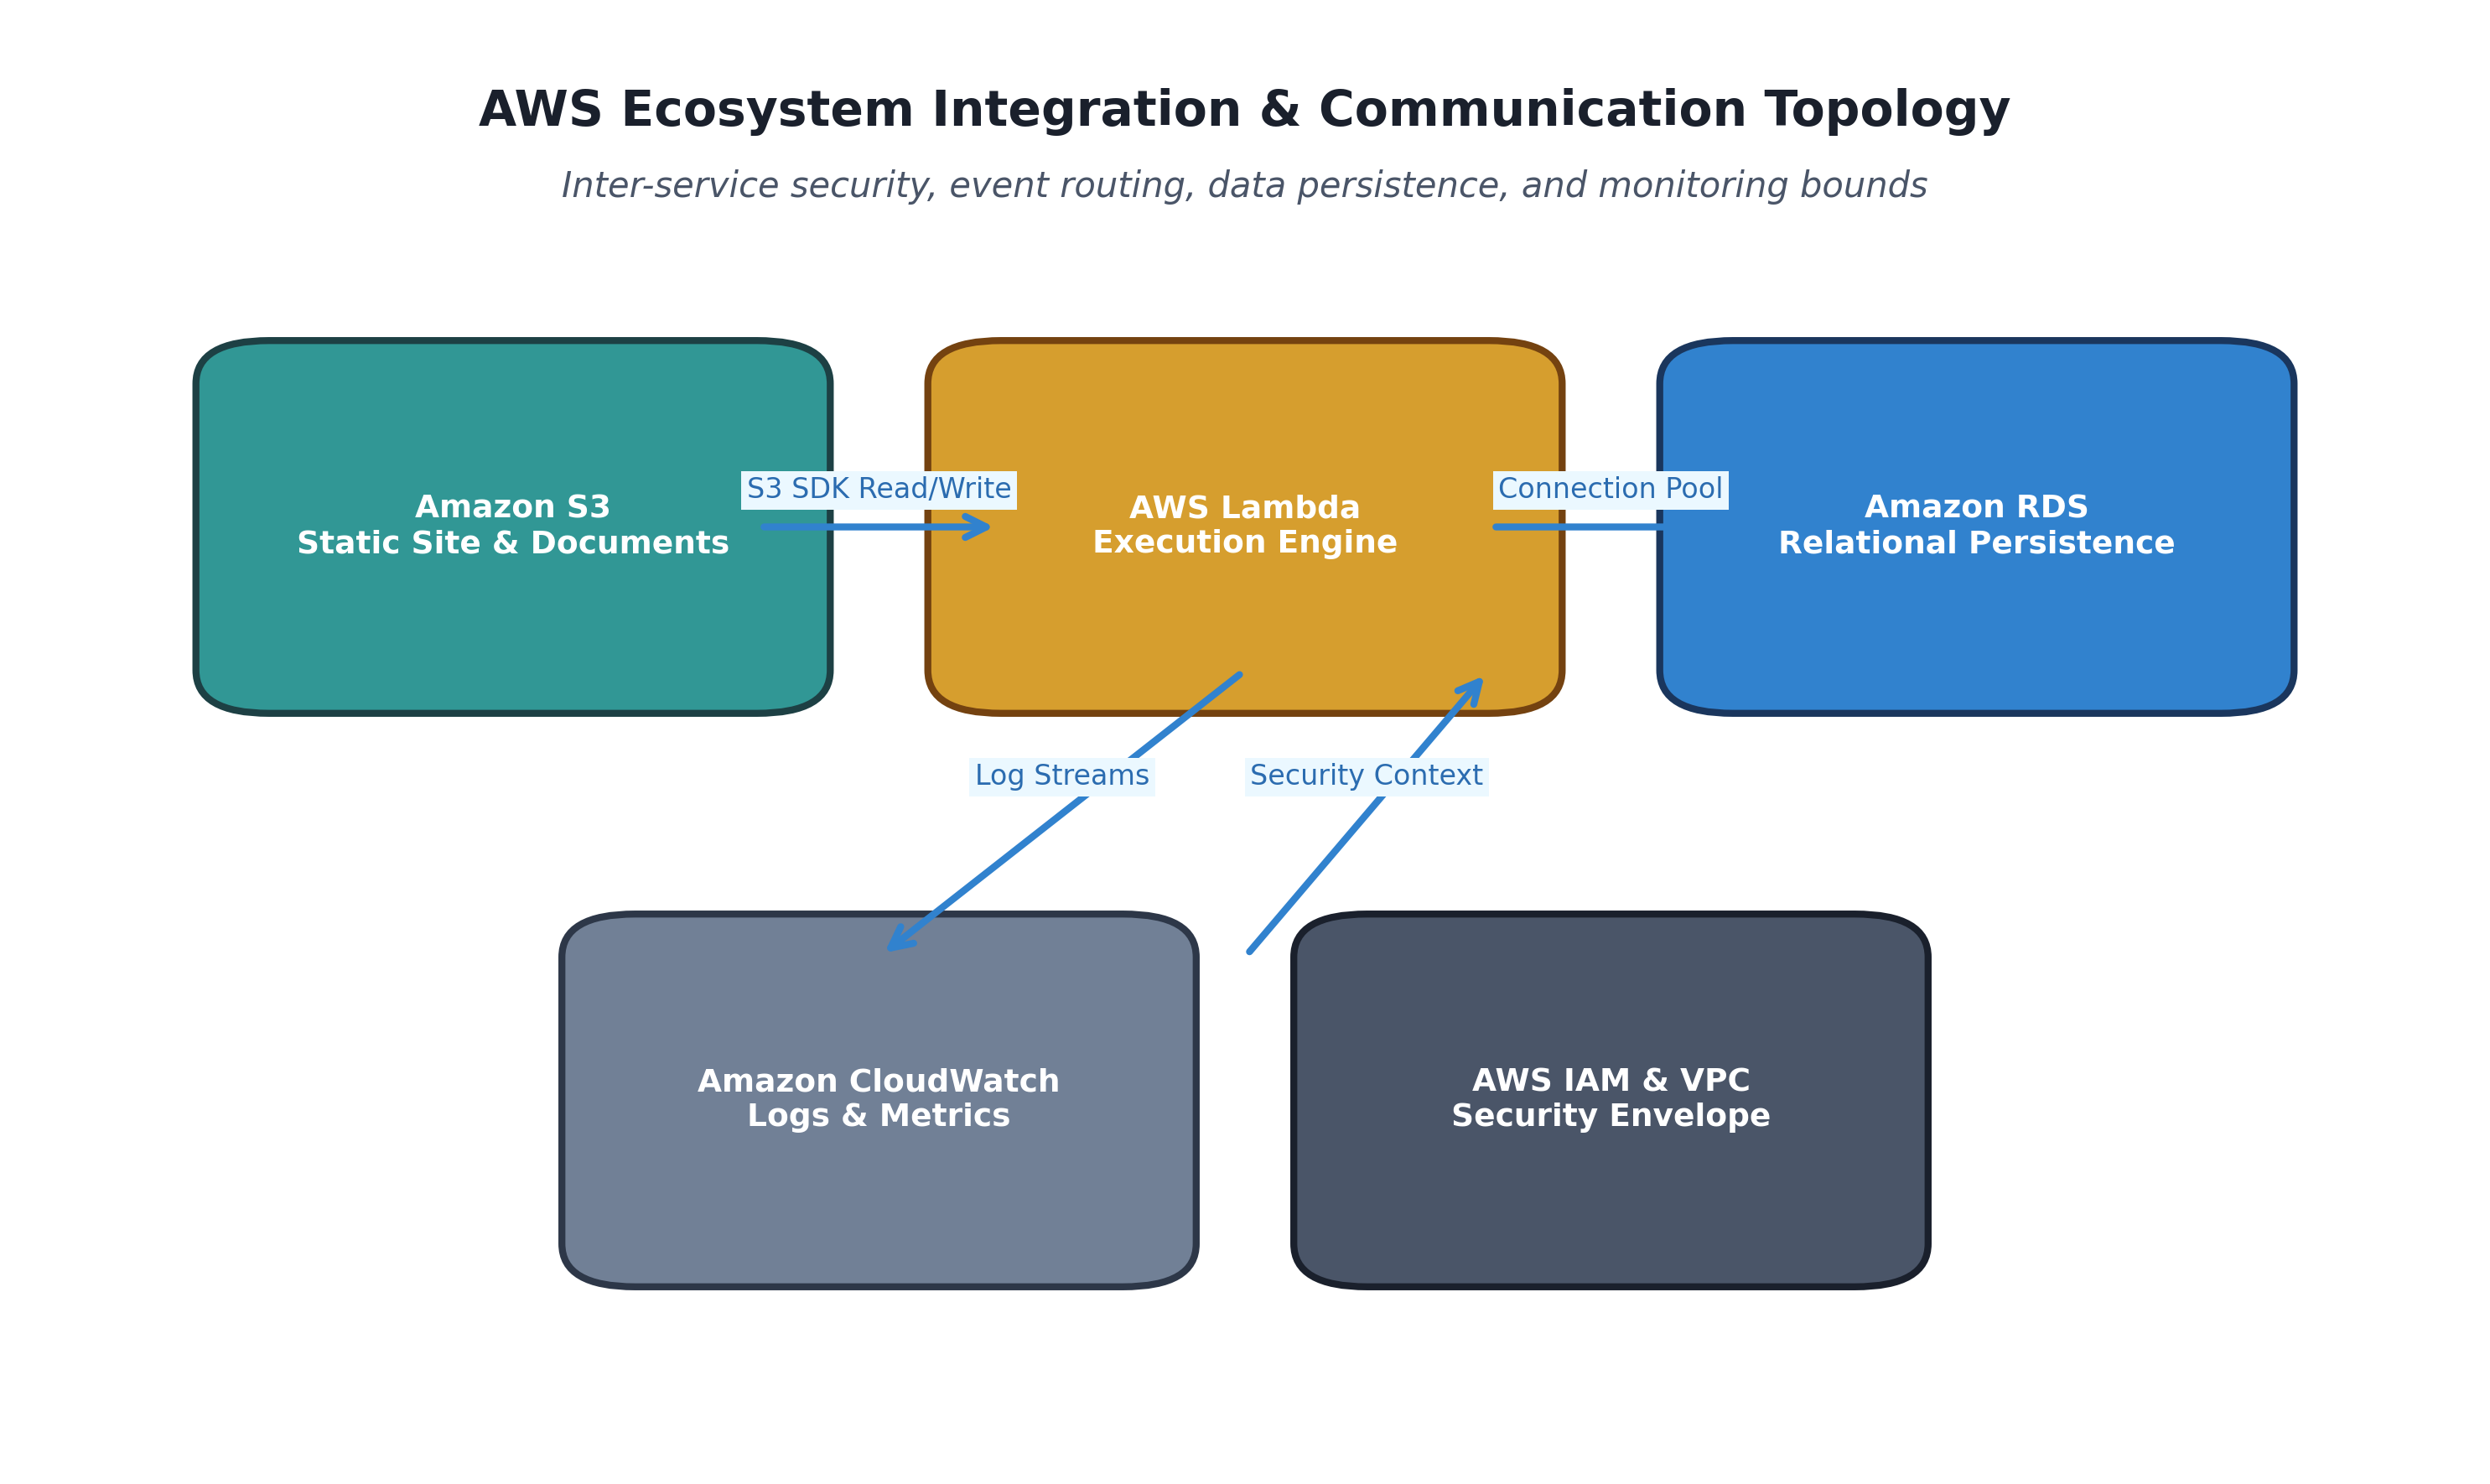
\includegraphics[width=0.88\textwidth]{figures/service_relationship.png}
\caption{AWS Ecosystem Inter-Service Communication and Security Topology}
\label{fig:service_rel}
\end{figure}
